\documentclass[a4paper,12pt]{article}

\usepackage{graphics}
\usepackage[pdftex]{graphicx}

%opening
\title{}
\author{}

\begin{document}

\section{Aper\c cu du logiciel}

\par
Le programme r\'ealis\'e pour \'etudier la structure de l'internet dipose de modules de lecture de donn\'ees et de calcul ainsi que d'une interface graphique. Pour pouvoir g\'erer au mieux tous ces \'el\'ements, il nous a paru opportun d'utiliser un mod\`ele vue-contr\^oleur.
\par
Le mod\`ele vue-contr\^oleur repose sur la s\'eparation des \'el\'ements de traitement de donn\'ees et des \'el\'ements de l'interface graphique. Le traitement des donn\'ees reste ind\'ependant de l'interface ce qui permet des modifications en toutes simplicit\'es. Un contr\^oleur sert de lien entre les deux parties. \\
Le sch\'ema suivant r\'esume le mod\`ele vue-contr\^oleur :

\begin{figure}[ht]
\centering
 \fbox
 {
 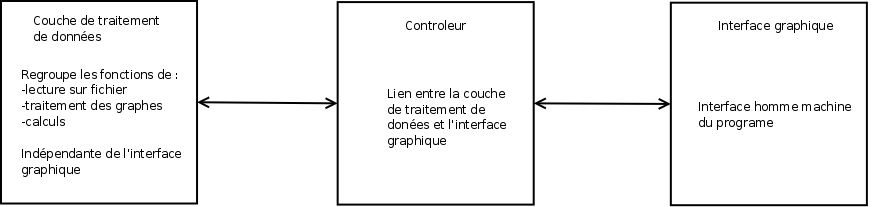
\includegraphics[width=16cm]{./schema/modele_mvc.png}
 }
  \caption{\label{mvc}Le mod\`ele vue-contr\^oleur}
\end{figure}




\end{document}
